\documentclass[11pt, a4paper, oneside]{article}
\usepackage[margin=1in]{geometry}    
\geometry{letterpaper}       
%\geometry{landscape}                % Activate for for rotated page geometry
\usepackage[parfill]{parskip}    % Deactivate to begin paragraphs with an indent rather than an empty line
\usepackage{amsfonts, amscd, amssymb, amsthm, amsmath}
\usepackage{pdfsync}  %leaves makers for tex searching
\usepackage{enumerate}
\usepackage{multicol}
\usepackage[pdftex,bookmarks]{hyperref}
\usepackage{enumitem}


\setlength\parindent{0pt}

%%% Theorems %%%--------------------------------------------------------- 
\theoremstyle{plain}
	\newtheorem{thm}{Theorem}[section]
	\newtheorem{lemma}[thm]{Lemma}
	\newtheorem{prop}[thm]{Proposition}
	\newtheorem{cor}[thm]{Corollary}
\theoremstyle{definition}
	\newtheorem*{defn}{Definition}
	\newtheorem{remark}{Remark}
\theoremstyle{example}
	\newtheorem*{example}{Example}


%%% Environments %%%--------------------------------------------------------- 
\newenvironment{ans}{\color{black}\medskip \paragraph*{\emph{Answer}.}}{\hfill \break  $~\!\!$ \dotfill \medskip }
\newenvironment{sketch}{\medskip \paragraph*{\emph{Proof sketch}.}}{ \medskip }
\newenvironment{summary}{\medskip \paragraph*{\emph{Summary}.}}{  \hfill \break  \rule{1.5cm}{0.4pt} \medskip }
\newcommand\Ans[1]{\color{black}\hfill \emph{Answer:} {#1}}


%%% Pictures %%%--------------------------------------------------------- 
%%% If you need to draw pictures, tikzpicture is one good option. Here are some basic things I always use:
\usepackage{tikz}
\usetikzlibrary{arrows}
\tikzstyle{V}=[draw, fill =black, circle, inner sep=0pt, minimum size=2pt]
\newcommand\TikZ[1]{\begin{matrix}\begin{tikzpicture}#1\end{tikzpicture}\end{matrix}}



%%% Color  %%%---------------------------------------------------------
\usepackage{color}
\newcommand{\blue}[1]{{\color{blue}#1}}
\newcommand{\NOTE}[1]{{\color{blue}#1}}
\newcommand{\MOVED}[1]{{\color{gray}#1}}


%%% Alphabets %%%---------------------------------------------------------
%%% Some shortcuts for my commonly used special alphabets and characters.
\def\cA{\mathcal{A}}\def\cB{\mathcal{B}}\def\cC{\mathcal{C}}\def\cD{\mathcal{D}}\def\cE{\mathcal{E}}\def\cF{\mathcal{F}}\def\cG{\mathcal{G}}\def\cH{\mathcal{H}}\def\cI{\mathcal{I}}\def\cJ{\mathcal{J}}\def\cK{\mathcal{K}}\def\cL{\mathcal{L}}\def\cM{\mathcal{M}}\def\cN{\mathcal{N}}\def\cO{\mathcal{O}}\def\cP{\mathcal{P}}\def\cQ{\mathcal{Q}}\def\cR{\mathcal{R}}\def\cS{\mathcal{S}}\def\cT{\mathcal{T}}\def\cU{\mathcal{U}}\def\cV{\mathcal{V}}\def\cW{\mathcal{W}}\def\cX{\mathcal{X}}\def\cY{\mathcal{Y}}\def\cZ{\mathcal{Z}}

\def\AA{\mathbb{A}} \def\BB{\mathbb{B}} \def\CC{\mathbb{C}} \def\DD{\mathbb{D}} \def\EE{\mathbb{E}} \def\FF{\mathbb{F}} \def\GG{\mathbb{G}} \def\HH{\mathbb{H}} \def\II{\mathbb{I}} \def\JJ{\mathbb{J}} \def\KK{\mathbb{K}} \def\LL{\mathbb{L}} \def\MM{\mathbb{M}} \def\NN{\mathbb{N}} \def\OO{\mathbb{O}} \def\PP{\mathbb{P}} \def\QQ{\mathbb{Q}} \def\RR{\mathbb{R}} \def\SS{\mathbb{S}} \def\TT{\mathbb{T}} \def\UU{\mathbb{U}} \def\VV{\mathbb{V}} \def\WW{\mathbb{W}} \def\XX{\mathbb{X}} \def\YY{\mathbb{Y}} \def\ZZ{\mathbb{Z}}  

\def\fa{\mathfrak{a}} \def\fb{\mathfrak{b}} \def\fc{\mathfrak{c}} \def\fd{\mathfrak{d}} \def\fe{\mathfrak{e}} \def\ff{\mathfrak{f}} \def\fg{\mathfrak{g}} \def\fh{\mathfrak{h}} \def\fj{\mathfrak{j}} \def\fk{\mathfrak{k}} \def\fl{\mathfrak{l}} \def\fm{\mathfrak{m}} \def\fn{\mathfrak{n}} \def\fo{\mathfrak{o}} \def\fp{\mathfrak{p}} \def\fq{\mathfrak{q}} \def\fr{\mathfrak{r}} \def\fs{\mathfrak{s}} \def\ft{\mathfrak{t}} \def\fu{\mathfrak{u}} \def\fv{\mathfrak{v}} \def\fw{\mathfrak{w}} \def\fx{\mathfrak{x}} \def\fy{\mathfrak{y}} \def\fz{\mathfrak{z}}
\def\fgl{\mathfrak{gl}}  \def\fsl{\mathfrak{sl}}  \def\fso{\mathfrak{so}}  \def\fsp{\mathfrak{sp}}  
\def\GL{\mathrm{GL}} \def\SL{\mathrm{SL}} \def\sl{\mathrm{sl}} \def\gl{\mathrm{gl}} \def\SO{\mathrm{SO}} \def\SU{\mathrm{SU}}  \def\SP{\mathrm{SP}} \def\g{\mathfrak{g}} \def\h{\mathfrak{h}} \def\Sym{\mathrm{Sym}}

\def\<{\langle} \def\>{\rangle}
\usepackage{mathabx}
\def\acts{\lefttorightarrow}
\def\ad{\mathrm{ad}} 
\def\Aut{\mathrm{Aut}}
\def\Ann{\mathrm{Ann}}
\def\dim{\mathrm{dim}} 
\def\End{\mathrm{End}} 
\def\ev{\mathrm{ev}} 
\def\Fr{\mathcal{F}\mathrm{r}}
\def\half{\hbox{$\frac12$}}
\def\Hom{\mathrm{Hom}} 
\def\id{\mathrm{id}} 
\def\sgn{\mathrm{sgn}}  
\def\supp{\mathrm{supp}}  
\def\Tor{\mathrm{Tor}}
\def\tr{\mathrm{tr}} 
\def\vep{\varepsilon}
\def\f{\varphi}
\def\image{\mathrm{Im}}


\def\Obj{\mathrm{Obj}}
\def\normeq{\unlhd}
\def\Set{{\cS\mathrm{et}}}
\def\Fin{{\cF\mathrm{inSet}}}
\def\Set{{\cS\mathrm{et}}}
\def\Grp{{\cG\mathrm{rp}}}
\def\Ab{{\cA\mathrm{b}}}
\def\Mod{{\cM\mathrm{od}}}
\def\ab{\mathrm{ab}}
\def\lcm{\mathrm{lcm}}
\def\ZZn{\ZZ/n\ZZ}


%%%%%%%%%%%%%%%%%%%%%%%%%%%%%% 
%%%%%%%%%%%%%%%%%%%%%%%%%%%%%%

\begin{document}
\title{Representation Theory of $\sl_n(\CC)$}
\author{Chris Hayduk}
\date{May 25, 2021}
\maketitle

\begin{abstract}
In this paper, we examine the representation theory of $\sl_n(\CC)$. In order to facilitate this discussion, we begin with an overview and deepening of our work with Lie groups and Lie algebras. Once the necessary background is in place, we move to discussing exterior and symmetric powers, Weyl's construction, and Cartan subalgebras. These three topics are used directly in the representation theory of $\sl_n(\CC)$, and so it is vital to have a strong understanding of them. Finally, we explicitly construct the representations of $\sl_n(\CC)$ using this background which we have built up.
\end{abstract}



%%%%%%%%%%%%%%%%%%%%%%%%%%%%%%%%%%%%%%%%%%%%%%%%%%%%%%%%%%%%%%%%%%%%%%%%%%%%%%%%%%%%%%%%%%%%%%%%%%%%%%%%%%%%%%%%%
%%%%%%%%%%%%%%%%%%%%%%%%%%%%%%%%%%%%%%%%%%%%%%%%%%%%%%%%%%%%%%%%%%%%%%%%%%%%%%%%%%%%%%%%%%%%%%%%%%%%%%%%%%%%%%%%%

\section{Introduction}

Representation theory is, generally speaking, the study of group actions on vector spaces \cite{fulton}. In this paper, we will be examining the representation theory of matrix Lie algebras of finite dimension. Lie algebras are the tangent spaces to Lie groups at the identity, and Lie groups are groups which are also differentiable manifolds \cite{liealgebrawiki, liegroupwiki}. These types of groups and algebras allow us to synthesize many of the concepts of analysis and algebra, opening up a wide range of applications and techniques.

\par
In this paper, we will be looking at the $n$-dimensional special linear group over the complex numbers, denoted by $\sl_n(\CC)$. This algebra in particular is of great importance in a number of areas. Firstly, it can be used as a model for studying other Lie algebras \cite{specialwiki}. Hence, it is important to understand its construction in order to become familiar with a wider array of Lie algebras. Moreover, $\sl_n(\CC)$ for $n = 2$ shows up in various physical contexts. We have that $\sl_2(\CC)$ is fundamental to the study of special relativity, general relativity, and supersymmetry \cite{specialwiki}. In particular, the adjoint representation of $\sl_2(\CC)$ generates the Lorentz group in special relativity \cite{specialwiki}. Hence, the representation theory of $\sl_n(\CC)$ is vital in a number of areas. In order to analyze this theory deeply, we first start by refreshing and deepening some background knowledge on Lie groups and Lie algebras. We then move to discussing background topics which will be used directly in the representation theory of $\sl_n(\CC)$. Finally, we explicitly construct the representations of $\sl_n(\CC)$.



%%%%%%%%%%%%%%%%%%%%%%%%%%%%%%%%%%%%%%%%%%%%%%%%%%%%%%%%%%%%%%%%%%%%%%%%%%%%%%%%%%%%%%%%%%%%%%%%%%%%%%%%%%%%%%%%%
%%%%%%%%%%%%%%%%%%%%%%%%%%%%%%%%%%%%%%%%%%%%%%%%%%%%%%%%%%%%%%%%%%%%%%%%%%%%%%%%%%%%%%%%%%%%%%%%%%%%%%%%%%%%%%%%%

\section{Refresher on Lie Groups and Lie Algebras}

\subsection{Lie Groups}

\subsubsection{Introduction}

Lie groups are groups which are also differentiable manifolds \cite{liegroupwiki}. A manifold is an object which locally resembles Euclidean space \cite{liegroupwiki}. For example, the surface of the sphere is not Euclidean, but if we zoom in enough, it begins to appear to be the Euclidean plane. As a group, Lie groups have a multiplicative operation as well as inverses \cite{liegroupwiki}. Moreover, as a Lie group, these operations are smooth. That is, group multiplication and the taking of inverses are differentiable in Lie groups \cite{liegroupwiki}. In this way, Lie groups provide us with a mixture of both algebraic and analytic concepts and interpretations.

\par
To make these notions more precise, let us define the concepts of manifold, smooth manifold, and Lie groups. Firstly, an $n$-dimensional \textbf{manifold} is an object $M$ which is a second-countable, Hausdorff topological space with the property that each $m \in M$ has a neighborhood that is homeomorphic to an open subset of $\RR^n$ \cite[\S 1.5]{hall}. As mentioned above, the surface of the sphere looks locally like $\RR^2$. That is, the neighborhood of any point $p$ on the surface of the sphere is homeomorphic to an open subset of $\RR^2$. However, the entire surface of the sphere is not homeomorphic to $\RR^2$. Now, a \textbf{smooth manifold} is a manifold $M$ together with a collection of local coordinates covering $M$ such that the change-of-coordinates map between two overlapping coordinate systems is smooth (that is, differentiable) \cite[\S 1.5]{hall}. Now we can define a Lie group \cite[\S 1.5, Definition 1.20]{hall}:

\par
\textbf{Definition.} A Lie group is a smooth manifold $G$ which is also a group such that the group product $$G \times G \to G$$ and the inverse map $G \to G$ are smooth.

\subsubsection{Matrix Lie Groups}

\par
The above general definition of a Lie group is useful, but we may limit our attention to \textit{matrix Lie groups}, as most of the canonical examples for Lie groups come from this space \cite[\S 1.1]{stillwell}. We must note, however, that not every Lie group is isomorphic to a matrix Lie group \cite[\S 1.5]{hall}.

\par
A matrix Lie group is a set of $n \times n$ matrices that is closed under products, inverses, and nonsingular limits \cite[\S 1.1]{stillwell}. The final condition, that of closure under nonsingular limits, simply means that if $A_1, A_2, A_3, \ldots$ is a convergent sequence of matrices in a Lie group $G$ and $A = \lim_{k \to \infty} A_k$ has an inverse, then $A \in G$ \cite[\S 1.1]{stillwell}. This condition is essentially equivalent to smoothness for matrix groups \cite[\S 1.1]{stillwell}.

\par
We can now give a couple of examples of matrix Lie groups in order to motivate these definitions and introduce some groups which we will be returning to later in this paper. Firstly, we have the general linear group, $\GL_n$. This group is usually taken over $\RR$ or $\CC$ - in  this case we will be taking $\GL_n(\CC)$, which is the the space of $n \times n$ invertible matrices with complex entries. We have that if $A_m$ is a sequence of matrices in $\GL_n(\CC)$ and $A_m$ converges to $A$ which has an inverse, then by the definition $\GL_n(\CC)$, we have $A \in \GL_n(\CC)$, hence showing that $\GL_n(\CC)$ is a matrix Lie group \cite[\S 1.2.1]{hall}. The special linear group $\SL_n(\CC)$ is the group of $n \times n$ invertible matrices having determinant $1$ with entries in $\CC$. If $A_n$ is a sequence of matrices with determinant one and $A_n$ converges to $A$, then $\det(A) = 1$ since determinant is a continuous function \cite[\S 1.2.1]{hall}. Hence, $\SL_n(\CC)$ is a matrix Lie group as well. 

\subsubsection{Connected Lie Groups}

We provide the following definition for a connected Lie group, which will be useful when considering Lie algebras \cite[\S 1.3.2, Definition 1.9]{hall}:

\par
\textbf{Definition.} A matrix Lie group $G$ is said to be connected if for all $A$ and $B$ in $G$, there exists a continuous path $A(t), a \leq t \leq b$, lying in $G$ with $A(a) = A$ and $A(b) = B$. For any matrix Lie group $G$, the identity component of $G$, denoted $G_0$, is the set of $A \in G$ for which there exists a continuous path $A(t), a \leq t \leq b$, lying in $G$ with $A(a) = I$ and $A(b) = A$.

\par
The above definition is really for path connectedness, but for matrix Lie groups, connectedness and path connectedness are equivalent concepts \cite[\S 1.3.2]{hall}.

\subsection{Lie Algebras}

\subsubsection{Introduction and Motivations}

Lie algebras are very closely related to Lie groups. In fact, we can derive a Lie algebra from any Lie group \cite{liealgebrawiki}. The Lie algebra of a Lie group is simply the tangent space at the identity of the group \cite{liealgebrawiki}. On the other hand, there is a corresponding connected Lie group for any finite-dimensional Lie algebra over $\RR$ or $\CC$ \cite{liealgebrawiki}. Hence, we can study the structure and classifications of Lie groups through their corresponding Lie algebras \cite{liealgebrawiki}.

\par
Expanding on our claim that the representations of Lie groups correspond to the representations of their Lie algebras, we have the following statement \cite[\S 8.1, Exercise 8.1]{fulton}:

\par
Let $G$ be a connected Lie group and $U \subset G$ any neighborhood of the identity. Then $U$ generates $G$.

\par
We are now starting to see why Lie algebras, as the tangent space at the identity of the Lie group, are able to contain so much information about the group. In fact, the above statement implies that any map between connected Lie groups $\rho: G \to H$ is fully determined by what it does on any open set containing the identity of $G$ \cite[\S 8.1]{fulton}. We can even make this notion stronger through the following principle \cite[\S 8.1]{fulton}:

\par
Let $G$ and $H$ be Lie groups, with $G$ connected. A map $\rho: G \to H$ is uniquely determined by its differential $d\rho_e: T_eG \to T_eH$ at the identity.

\par
Again, we can see that we are getting closer to the notion that representations of Lie algebras are equivalent to those of the underlying groups. Now that we have the motivation and intuitions regarding Lie algebras, we will present some definitions and examples to make these notions more rigorous.

\subsubsection{Basic Definitions}

The explicit definition of a Lie algebra $\mathfrak{g}$ is as follows \cite[\S 8.1, Definition 8.9]{fulton}:

\par
\textbf{Definition.} A Lie algebra $\mathfrak{g}$ is a vector space together with a skew-symmetric bilinear map $$[,]: \mathfrak{g} \times \mathfrak{g} \to \mathfrak{g}$$ satisfying the Jacobi identity.

\par
Recall that skew symmetric is:
\begin{align*}
[x,y] = -[y,x]
\end{align*}

and that the Jacobi identity is given by:
\begin{align*}
[x, [y,z]] + [y,[z,x]] + [z,[x,y]] = 0
\end{align*}

To sum up the work so far \cite[\S 8.1]{fulton}:
\begin{enumerate}
\item the tangent space $\mathfrak{g}$ at the identity to a Lie group $G$ is naturally endowed with the structure of a Lie algebra;
\item if $G$ and $H$ are Lie groups with $G$ connected, the maps from $G$ to $H$ are in one-to-one correspondence with maps of the associated Lie algebras, by associating to $\rho: G \to H$ its differential $(d\rho)_e: \mathfrak{g} \to \mathfrak{h}$.
\end{enumerate}

Building off of these notions, we can now define a representation of a Lie algebra \cite[\S 8.1]{fulton}:

\par
\textbf{Definition.} A \textit{representation} of a Lie algebra $\mathfrak{g}$ on a vector space $V$ is simply a map of Lie algebras $$\rho: \mathfrak{g} \to \End(V)$$ i.e., a linear map that preserves brackets, or an action of $\mathfrak{g}$ on $V$ such that $$[X, Y](v) = X(Y(v)) - Y(X(v))$$

The above definition, alongside statement $2$ from our summary of the work so far above, we have that representation of a connected Lie group are in one-to-one correspondence with representations of its Lie algebras \cite[\S 8.1]{fulton}.


\subsubsection{Lie Algebra of a Matrix Lie Group}

We can now drill down to matrix Lie groups from general Lie groups. The following provides a definition for a Lie algebra over a matrix Lie group \cite[\S 3.3, Definition 3.18]{hall}:

\par
\textbf{Definition.} Let $G$ be a matrix Lie group. The Lie algebra of $G$, denoted $\mathfrak{g}$, is the set of all matrices $X$ such that $e^{tX}$ is in $G$ for all real numbers $t$.

\par
We have that, similar to the case of general Lie groups, $\mathfrak{g}$ is the tangent space to $G$ at the identity \cite[\S 3.3]{hall}. We can now present some examples of Lie algebras, particularly $\sl_n(\CC)$, which we will discuss the representation theory of in the next section. We present the following proposition to give some examples these \cite[\S 3.4, Proposition 3.23]{hall}:

\par
\textbf{Proposition.} The Lie algebra of $\GL_n(\CC)$ is the space $M_n(\CC)$ of all $n \times n$ matrices with complex entries. Similarly, the Lie algebra of $\GL_n(\RR)$ is equal to $M_n(\RR)$. The Lie algebra of $\SL_n(\CC)$ consists of $n \times n$ complex matrices with trace zero, and the Lie algebra of $\SL_n(\RR)$ consists of all $n \times n$ real matrices with trace zero.

\par
We denote the Lie algebras of these groups as $\gl_n(\CC)$, $\gl_n(\RR)$, $\sl_n(\CC)$, and $\sl_n(\RR)$.

\begin{proof}
If $X \in M_n(\CC)$, then $e^{tX}$ is invertible, so that $X$ belongs to the Lie algebra of $\GL_n(\CC)$. If $X \in M_n(\RR)$, then $e^{tX}$ is invertible and real, so that $X$ is in the Lie algebra of $\GL_n(\RR)$. Conversely, if $e^{tX}$ is real for all real $t$, then $X = d(e^{tX})/dt |_{t = 0}$ must also real. If $X \in M_n(\CC)$ has trace zero, then $\det(e^{tX} = 1$, showing that $X$ is in the Lie algebra of $\SL_n(\CC)$. Conversely, if $\det(e^{tX}) = e^{t \cdot \tr(X)} = 1$ for all real $t$, then,
\begin{align*}
\tr(X) = \frac{d}{dt} e^{t \cdot \tr(X)} \rvert_{t=0} = 0
\end{align*}

Finally, if $X$ is real and has trace zero, then $e^{tX}$ is real and has determinant $1$ for all real $t$, showing that $X$ is in the Lie algebra of $\SL_n(\RR)$. Conversely, if $e^{tX}$ is real and has determinant $1$ for all real $t$, the preceding arguments show that $X$ must be real and have trace $0$.
\end{proof}


%%%%%%%%%%%%%%%%%%%%%%%%%%%%%%%%%%%%%%%%%%%%%%%%%%%%%%%%%%%%%%%%%%%%%%%%%%%%%%%%%%%%%%%%%%%%%%%%%%%%%%%%%%%%%%%%%
%%%%%%%%%%%%%%%%%%%%%%%%%%%%%%%%%%%%%%%%%%%%%%%%%%%%%%%%%%%%%%%%%%%%%%%%%%%%%%%%%%%%%%%%%%%%%%%%%%%%%%%%%%%%%%%%%

\section{Representation Theory of $\sl_n(\CC)$}

\subsection{Background Information}

In order to fully analyze the representation theory of $\sl_n(\CC)$, we will need to introduce some additional concepts which we will make use of in our analysis.

\subsubsection{Exterior and Symmetric Powers}

Exterior powers will be used extensively in our analysis of $\sl_n(\CC)$. They can be defined as follows \cite[\S B.2]{fulton}:

\par
\textbf{Definition.} The exterior powers $\bigwedge^n V$ of a vector space $V$ come equipped with an alternating multilinear map $$V \times \cdots \times V \to \bigwedge^nV, \; \; \; \; v_1 \times \cdots v_n \mapsto v_1 \wedge \cdots \wedge v_n$$ that is universal. For $\beta: V \times \cdots \times V \to U$, an alternating multilinear map, there is a unique linear map from $\bigwedge^n V$ to $U$ which takes $v_1 \wedge \cdots \wedge v_n$ to $\beta(v_1 ,\ldots, v_n)$.

\par
This definition fully charactertizes the exterior powers of a vector space. We can now expand this definition in order to relate the tensor products of vector spaces to their exterior powers \cite[\S B.2]{fulton}:

\par
The exterior power can be constructed as the quotient space of $V^{\otimes n}$ by the subspace generated by all $v_1 \otimes \cdots \otimes v_n$ with two of the vectors equal. We let $$\pi: V^{\otimes n} \to \bigwedge^n V, \; \; \; \pi(v_1 \otimes \cdots \otimes v_n) = v_1 \wedge \cdots \wedge v_n$$ denote the projection. If $\{e_i\}$ is a basis for $V$, then $$\{e_{i_1} \wedge e_{i_2} \wedge \cdots \wedge e_{i_n}: i_1 < i_2 < \cdots < i_n\}$$ is basis for $\bigwedge^n V$.

\par
Lastly, we have that there exists an isomorphism such that \cite[\S B.2]{fulton}: $$\bigwedge^n(V \oplus W) \cong \bigoplus^n_{a = 0} \bigwedge^a V \oplus \bigwedge^{n-a} W$$ The isomorphism is given by a linear map from $\bigwedge^a V \otimes \bigwedge^b W$ to $\bigwedge^{a+b}(V \oplus W)$, which takes $(v_1 \wedge \cdots \wedge v_a) \otimes (w_1 \wedge \cdots \wedge w_b)$ to $v_1 \wedge \cdots \wedge v_a \wedge w_1 \wedge \cdots \wedge w_b$

\par
We have now defined exterior powers of vector spaces and given some important relations between exterior powers and tensor products of vectors spaces. We can thus now direct our attention to symmetric power \cite[\S B.2]{fulton}:

\par
\textbf{Definition.} The symmetric powers $\Sym^n V$ comes with a universal symmetric multilinear map $$V \times \cdots V \to \Sym^nV, \; \; \; \; v_1 \times \cdots \times v_n \mapsto v_1 \cdot \cdots \cdot v_n$$  The symmetric power can be constructed as the quotient space of $V^{\otimes n}$ by the subspace generated by all $v_1 \otimes \cdots \otimes v_n - v_{\sigma(1)} \otimes \cdots \otimes v_{\sigma(n)}$, or by those in which $\sigma$ permutes two successive factors. Again we let $$\pi: V^{\otimes n} \to \Sym^n V \; \; \; \; \pi(v_1 \otimes \cdots \otimes v_n) = v_1 \cdot \cdots \cdot v_n$$ denote the projection. If $\{e_i\}$ is a basis for $V$, then $$\{e_{i_1} \cdot e_{i_2} \cdot \cdots \cdot e_{i_n}: i_1 \leq i_2 \leq \cdots i_n\}$$ is a basis for $\Sym^n V$

\subsubsection{Weyl's Construction}

We'll present here some definitions and theorems without proof regarding Weyl's construction, which will be used in our analysis of $\sl_n(\CC)$. First, we begin with the definition of Weyl's construction. Consider the symmetric group $S_n$ acting on $V^{\otimes n}$, where $V$ is a vector space. We can permute the factors on the right like so, $$(v_1 \otimes \cdots \otimes v_d) \cdot \sigma = v_{\sigma(1)} \otimes \cdots \otimes v_{\sigma(d)}$$ Then this action commutes with the left action of $\GL(V)$. For any partition $\lambda$ of $n$, we have a Young symmetrizer $c_{\lambda}$ in $\CC S_n$ \cite[\S 6.1]{fulton}. We can define a Young symmetrizer as follows \cite{youngwiki}:

\par
\textbf{Definition.} A Young symmetrizer is an element of the group algebra of the symmetric group, constructed in such a way that, for the homomorphism from the group algebra to the endomorphisms of a vector space $V^{\otimes n}$ obtained from the action of $S_n$ on $V^{\otimes n}$ by permutation of the indices, the image of the endomorphism determined by that element corresponds to an irreducible representation of the symmetric group over the complex numbers. In particular, if we have a Young tableau $\lambda$ corresponding to a numbered partition of $n$ and consider the action of $S_n$ given by permuting the boxes of $\lambda$, we can define two permutation subgroups $P_{\lambda}$ and $Q_{\lambda}$ of $S_n$ as follows: $$P_{\lambda} = \{g \in S_n: g \text{ preserves each row of } \lambda\}$$ and $$Q_{\lambda} = \{g \in S_n: g \text{ preserves each column of } \lambda\}$$ Corresponding to these two subgroups, define two vectors in the group algebra $\CC S_n$ by $$a_{\lambda} = \sum_{g \in P_{\lambda}} e_g$$ and $$b_{\lambda} = \sum_{g \in Q_{\lambda}} \sgn(g) e_g$$ where $e_g$ is the unit vector corresponding to $g$ and $\sgn(g)$ is the sign of the permutation. Then the Young symmetrizer corresponding to the Young tableau $\lambda$ is given by the following product, $$c_{\lambda} := a_{\lambda}b_{\lambda} = \sum_{g \in P_{\lambda}, h \in Q_{\lambda}} \sgn(h) e_{gh}$$ Now, a Young tableau is a combinatorial object useful in representation theory which provides a convenient way to describe the group representations of the symmetric and general linear groups and to study their properties \cite{tableauwiki}. We provide an image of an example of a Young tableau for the reader to familiarize themselves with the object \cite{tableauwiki}:

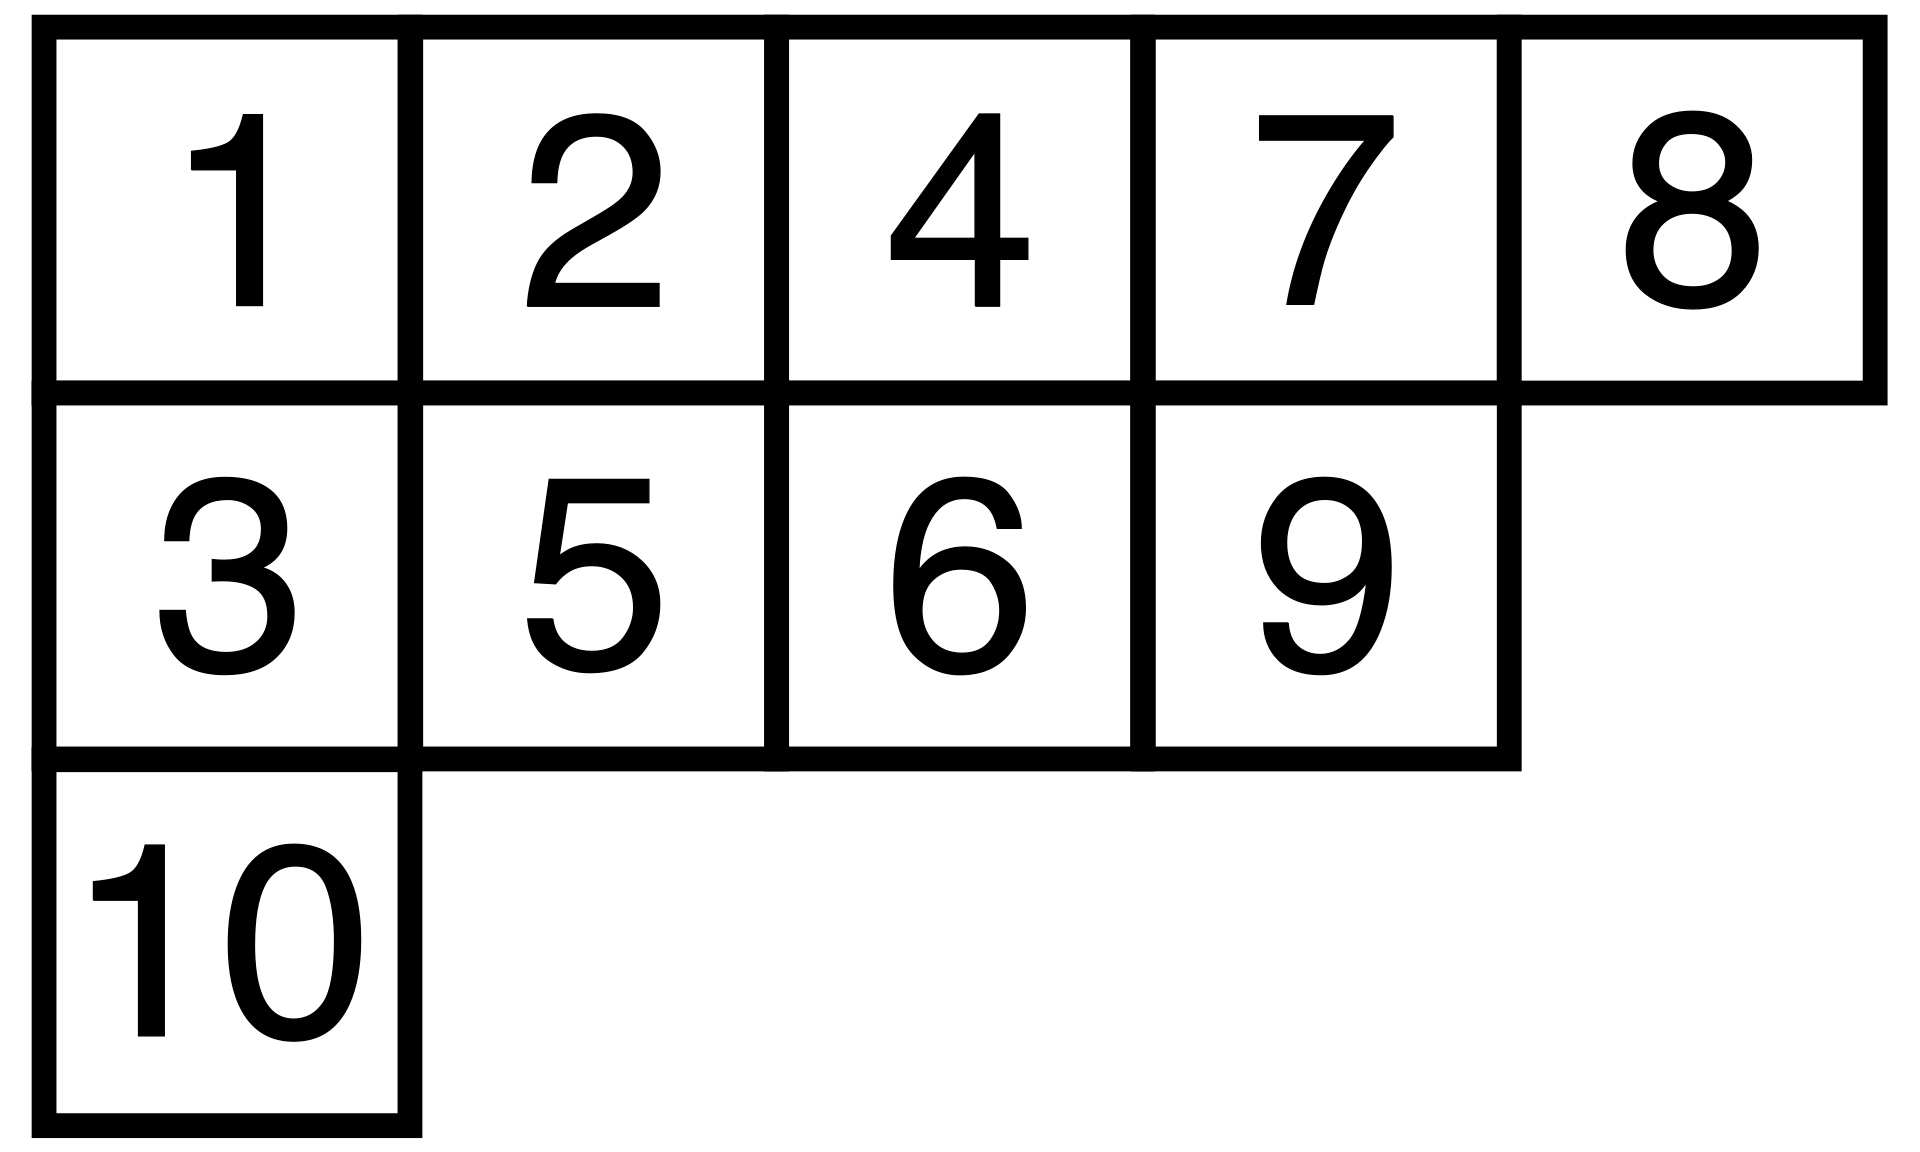
\includegraphics[scale=0.1]{young_tableau}

The definition given above is incredibly information dense and can be a bit difficult to parse. Essentially, we are giving ourselves a convenient way to compute irreducible representations of $S_n$ in $\CC S_n$. Now, back to Weyl's construction. We want to denote the image of $c_{\lambda}$ on $V^{\otimes n}$ by $\SS_{\lambda} V$ as \cite[\S 6.1]{fulton}: $$\SS_{\lambda} V = \image(c_{\lambda} |_{V^{\otimes n}})$$ which is a representation of $\GL(V)$. We can define Weyl's construction as follows \cite[\S 6.1]{fulton}:

\par
\textbf{Definition.} We call the functor $V \rightsquigarrow \SS_{\lambda} V$ Weyl's construction corresponding to $\lambda$.

\par
The above definition being a functor means that a linear map $\varphi: V \to W$ of vector spaces determines a linear map $\SS_{\lambda}(\varphi): \SS_{\lambda} V \to \SS_{\lambda} W$ with $\SS_{\lambda}(\varphi \circ \psi) = \SS_{\lambda}(\varphi) \circ \SS_{\lambda}(\psi)$ and $\SS_{\lambda}(\id_V) = \id_{\SS_{\lambda} V}$ \cite[\S 6.1]{fulton}.

\par
Now that we have presented the necessary background and definition of Weyl's construction, we will present a theorem and corollary which will help to expand the uses of this idea \cite[\S 6.1, Theorem 6.3]{fulton}:

\par
\textbf{Theorem.} \begin{enumerate}
\item Let $k = \dim V$. Then $\SS_{\lambda} V$ is zero if $\lambda_{k+1} \neq 0$. If $\lambda = (\lambda_1 \geq \cdots \geq \lambda_k \geq 0)$, then $$\dim \SS_{\lambda} V = S_{\lambda}(1, \cdots, 1) = \prod_{1 \leq i< j \leq k} \frac{\lambda_i - \lambda_j + j - i}{j-i}$$
\item Let $m_{\lambda}$ be the dimension of the irreducible representation $V_{\lambda}$ of $S_n$ corresponding to $\lambda$. Then $$V^{\otimes n} \cong \bigoplus_{\lambda} \SS_{\lambda} V^{\otimes m_{\lambda}}$$
\item For any $g \in \GL(V)$, the trace of $g$ on $\SS_{\lambda} V$ is the value of the Schur polynomial on the eigenvalues $x_1, \ldots, x_k$ of $g$ on $V$: $$\chi_{\SS_{\lambda}V}(g) = S_{\lambda}(x_1, \ldots, x_k)$$
\item Each $\SS_{\lambda} V$ is an irreducible representation of $\GL(V)$.
\end{enumerate}

And the corollary is as follows \cite[\S 6.1, Corollary 6.6]{fulton}:

\par
\textbf{Corollary.} If $c \in \CC S_n$ and $(\CC S_n) \cdot c = \bigoplus_{\lambda} V_{\lambda}^{\oplus r_{\lambda}}$ as representations of $S_n$, then there is a corresponding decomposition of $\GL(V)$-spaces: $$V^{\otimes n} \cdot c = \bigoplus_{\lambda} \SS_{\lambda} V^{\oplus r_{\lambda}}$$ If $x_1, \ldots, x_k$ are the eigenvalues of an endomorphism of $V$, the trace of the induced endomorphism of $V^{\otimes n} \cdot c$ is $\sum r_{\lambda} S_{\lambda}(x_1, \ldots, x_k)$

\subsubsection{Cartan Subalgebras}

We have that a Cartan subalgebra is a nilpotent subalgebra $\mathfrak{h}$ of a Lie algebra $\mathfrak{g}$ that is self-normalizing (if $[X, Y] \in \mathfrak{h}$ for all $X \in \mathfrak{h}$, then $Y \in \mathfrak{h}$) \cite{cartanwiki}. We have that a nilpotent Lie algebra is a Lie algebra $\mathfrak{g}$ with a lower central series which terminates in the zero subalgebra. That is, the following sequence of subalgebras arrives at the zero subalgebra eventually \cite{nilpotentwiki}: $$\g \geq [\g, \g] \geq [\g, [\g, \g]] \geq [\g, [\g, [\g, \g]]] \geq \cdots$$

That is, $\g_n = 0$ for some $n \in \NN$.

\par
Cartan subalgebras are introduced here because for finite dimensional semisimple Lie algebras defined over an algebraically closed field (which exactly characterizes $\sl_n(\CC)$), a Cartan subalgebra is equivalent to the maximal abelian subalgebra consisting of elements $x$ such that the adjoint endomorphism $\ad(x): \g \to \g$ is semisimple and thus diagonalizable \cite{cartanwiki}.

\par
Note that the adjoint representation of a Lie algebra $\g$ and a fixed $x \in \g$ is defined as the map,
\begin{align*}
\ad_x: \g \to \g \; \; \; \text{with} \; \; \; \ad_x(y) = [x, y]
\end{align*}

for all $y \in \g$ \cite{adjointwiki}.

\subsection{Analyzing Simple Lie Algebras}

The analysis of simple Lie algebras is broken down into seven steps by Fulton \cite[\S 14.1]{fulton}:
\begin{enumerate}
\item Verify that your Lie algebra is semisimple
\item Find an abelian subalgebra $\h \subset \g$ acting diagonally
\item Let $\h$ act on $\g$ by the adjoint representation, and decompose $\g$ accordingly
\item Find the distinguished subalgebras $\mathfrak{s}_{\alpha} \cong \sl_2(\CC) \subset \g$
\item Use the integrality of the eigenvalues of the $H_{\alpha}$ ($H_{\alpha} \in [\g_{\alpha}, \g_{-\alpha}]$ and $\alpha(H_{\alpha}) = 2$ where $\alpha \in \h^*$)
\item Use the symmetry of the eigenvalues of $H_{\alpha}$
\item Choose a direction in $\h*$
\item Classify the irreducible, finite-dimensional representations of $\g$
\end{enumerate}

These analysis steps culminate in the following theorem \cite[\S 14.1, Theorem 14.18]{fulton}:

\par
\textbf{Theorem.} For any $\alpha$ in the intersection of the Weyl chamber $\mathcal{W}$ associated to the ordering of the roots with the weight lattice $\Lambda_W$, there exists a unique, irreducible, finite-dimensional representation $\Gamma_{\alpha}$ of $\g$ with highest weight $\alpha$; this gives a bijection between $\mathcal{W} \cap \Lambda_W$ and the set of irreducible representations of $\g$. The weights of $\Gamma_{\alpha}$ will consist of those elements of the weight lattice congruent to $\alpha$ modulo the root lattice $\Lambda_R$ and lying in the convex hull of the set of points in $\h^*$ conjugate to $\alpha$ under the Weyl group.

\subsection{Analyzing $\sl_n(\CC)$}

We now have the necessary background to analyze the representations of $\sl_n(\CC)$. We must begin by finding a Cartan subalgebra. A choice of the subalgebra of diagnoal matrices works well \cite[\S 15.1]{fulton}. We write $H_i$ to denote the diagonal matrix $E_{i,i}$ which is the identity for $e_i$ and takes $e_j$ to $0$ for all $j \neq i$ \cite[\S 15.1]{fulton}. Thus, we have that \cite[\S 15.1]{fulton}: $$\mathfrak{h} = \{a_1H_1 + a_2H_2 + \cdots + a_nH_n: a_1 + a_2 + \cdots + a_n = 0\}$$ We can also write $$\h^* = \CC\{L_1, L_2, \ldots, L_n\}/(L_1 + L_2 + \cdots + L_n = 0)$$ where $L_i(H_i) = \delta_{i ,j}$ \cite[\S 15.1]{fulton}. $L_i$ is written for the image of $L_i$ in $\h^*$. If we consider $E_{i, j}$, which maps $e_i$ to $e_j$ and maps $e_k$ to $0$ for all $k \neq j$, we have \cite[\S 15.1]{fulton}: $$\ad(a_1 H_1 + a_2 H_2 + \cdots + a_n H_n)(E_{i,j}) = (a_i - a_j) \cdot E_{i,j}$$ Hence, we have that $E_{i,j}$ is eigenvector of the action on $\mathfrak{h}$ with eigenvalue $(L_i - L_j)$ \cite[\S 15.1]{fulton}. Thus, the roots of $\sl_n(\CC)$ are the pairwise difference of the $L_i$ \cite[\S 15.1]{fulton}. Since the roots are the pairwise differences of the vertices $L_i$, the root lattice $\Lambda_R$ generated by these roots can be characterized as $\Lambda_R = \{\sum a_i L_i: a_i \in \ZZ, \sum a_i = 0\}/(\sum L_i = 0)$ \cite[\S 15.1]{fulton}.

\par
The weight lattice of $\sl_n \CC$ may be realized as the lattice generated by the vertices of a regular $(n-1)$-simplex $\delta$ centered at the origin, and the roots as the pairwise differences of these vertices \cite[\S 15.1]{fulton}. Hence, the Weyl group is as follow \cite[\S 15.1]{fulton}:

\par
The reflection in the hyperplane perpendicular to the root $L_i - L_j$ will exchange  $L_i$ and $L_j$ in $\h^*$ and leave the other $L_k$ alone so that the Weyl group $\mathfrak{W}$ is just the group $S_n$ acting as the symmetric group on the generators $L_i$ of $\h^*$.


\par
We can index the irreducible representations of $\sl_n(\CC)$ nicely \cite[\S 15.1]{fulton}. For an arbitrary $(n-1)$-tuple of natural numbers $(a_1, \ldots, a_{n-1}) \in \NN^{n-1}$ we will denote by $\Gamma_{a_1, \ldots, a_{n-1}}$ the irreducible representation of $\sl_n(\CC)$ with highest weight $a_1 L_1 + a_2 (L_1 + L_2) + \cdots + a_{n-1} (L_1 + \cdots + L_{n-1}) = (a_1 + \cdots + a_{n-1}) L_1 + (a_2 + \cdots + a_{n-1}) L_2 + \cdots + a_{n-1} L_{n-1}$ \cite[\S 15.1]{fulton}: $$\Gamma_{a_1, \ldots, a_{n-1}} = \Gamma_{a_1 L_1 + a_2 (L_1 + L_2) + \cdots + a_{n-1} (L_1 + \cdots + L_{n-1}}$$

Moreover, when we locate the irreducible representations of $V^{(i)}$ with the highest weight $L_1 + \cdots + L_i$, the general irreducible representation $\Gamma_{a_1, \ldots, a_{n-1}}$ with highest weight $\sum a_i (L_1 + \cdots + L_i)$ will occur inside the tensor product of symmetric powers, $$\Sym^{a_1}V^{(1)} \otimes \Sym^{a_2}V^{(2)} \otimes \cdots \otimes \Sym^{a_{n-1}} V^{(n-1)}$$ of these representations \cite[\S 15.1]{fulton}. Hence, we simply need to find the basic representations of $V^{(i)}$ \cite[\S 15.1]{fulton}.

\par
Equivalently to the above, as discussed previously, we have that the irreducible representation $\Gamma_{a_1, \ldots, a_{n-1}}$ of $\sl_n(\CC)$ with highest weight $\sum a_i (L_1 + \cdots + L_i)$ will occur inside $V^{\otimes d}$ of the standard representation $V$ \cite[\S 15.3]{fulton}.

\par
We will now make use of Schur functors in order to construct the irreducible representation for $\sl_n(\CC)$. If we consider a partition of $V = \CC^n$ given by $$\lambda: \lambda_1 \geq \lambda_1 \geq \cdots \geq \lambda_1 \geq 0$$ we can apply the Schur functor $\mathbb{S}_{\lambda}(V) = \mathbb{S}_{\lambda}(\CC^n)$ in order to get a representation of $\GL_n(\CC)$ \cite[\S 15.3]{fulton}. Taking $d = \sum \lambda_i$, this is given by, $$\mathbb{S}_{\lambda} = V^{\otimes d}\cdot c_{\lambda} = V^{\otimes d} \otimes_{\CC S_d} V_{\lambda}$$ where $c_{\lambda}$ is the Young symmetrizer which we discussed previously and $V_{\lambda}$ is the irreducible representation of $S_d$ corresponding to $\lambda$ \cite[\S 15.3]{fulton}. Since $\mathbb{S}_{\lambda}V$ is an irreducible representation of $\GL_n(\CC)$, we have that it must be an irreducible representation of $\SL_n(\CC)$ as well \cite[\S 15.3]{fulton}. This gives rise to the following proposition \cite[\S 15.3, Proposition 15.15]{fulton}:

\par
\textbf{Proposition.} The representation $\mathbb{S}_{\lambda}(\CC^n)$ is the irreducible representation of $\sl_n(\CC)$ with highest weight $\lambda_1 L_1 + \lambda_2 L_2 + \cdots + \lambda_n L_n$.


%%%%%%%%%%%%%%%%%%%%%%%%%%%%%%%%%%%%%%%%%%%%%%%%%%%%%%%%%%%%%%%%%%%%%%%%%%%%%%%%%%%%%%%%%%%%%%%%%%%%%%%%%%%%%%%%%
%%%%%%%%%%%%%%%%%%%%%%%%%%%%%%%%%%%%%%%%%%%%%%%%%%%%%%%%%%%%%%%%%%%%%%%%%%%%%%%%%%%%%%%%%%%%%%%%%%%%%%%%%%%%%%%%%

\section{Conclusion}

In summary, we have described Lie groups and Lie algebras and analyzed the representation theory of one of the most prominent Lie algebras, $\sl_n$. Constructing these representations required a significant amount of background work, but now allows us simply characterize the ways in which $\sl_n$ acts on vector spaces. The algebra $\sl_n(\CC)$ is frequently used in the study of other Lie algebras \cite{specialwiki}. Moreover, it is quite important, in the form of $\sl_2(\CC)$, for the study of special relativity and general relativity \cite{specialwiki}. In particular, the adjoint representation of $\sl_2(\CC)$ generates the Lorentz group of special relativity, which plays a key role in many of the laws governing Minkowski spacetime \cite{specialwiki}. Hence, as discussed previously, the construction of these representations is of great mathematical and physical importance.

\newpage
\begin{thebibliography}{9}

\bibitem{adjointwiki}
“Adjoint Representation.” \textit{Wikipedia}, Wikimedia Foundation, 16 Apr. 2021, \\ en.wikipedia.org/wiki/Adjoint\_representation. 

\bibitem{cartanwiki}
“Cartan Subalgebra.” \textit{Wikipedia}, Wikimedia Foundation, 16 Apr. 2021, \\ en.wikipedia.org/wiki/Cartan\_subalgebra. 

\bibitem{fulton}
Fulton, William, and Joe Harris. \textit{Representation Theory: A First Course}. Springer, 2004. 

\bibitem{hall}
Hall, Brian C. \textit{Lie Groups, Lie Algebras, and Representations: An Elementary Introduction}. Springer, 2016.  

\bibitem{liealgebrawiki}
“Lie Algebra.” \textit{Wikipedia}, Wikimedia Foundation, 16 Apr. 2021, \\ en.wikipedia.org/wiki/Lie\_algebra. 

\bibitem{liegroupwiki}
“Lie Group.” \textit{Wikipedia}, Wikimedia Foundation, 21 Apr. 2021, \\ en.wikipedia.org/wiki/Lie\_group. 

\bibitem{nilpotentwiki}
“Nilpotent Lie Algebra.” \textit{Wikipedia}, Wikimedia Foundation, 21 Apr. 2021, \\ en.wikipedia.org/wiki/Nilpotent\_Lie\_algebra. 

\bibitem{specialwiki}
“Special Linear Lie Algebra.” \textit{Wikipedia}, Wikimedia Foundation, 16 Apr. 2021, \\ en.wikipedia.org/wiki/Special\_linear\_lie\_algebra. 

\bibitem{stillwell}
Stillwell, John. \textit{Naive Lie Theory}. Springer, 2012.

\bibitem{tableauwiki}
“Young Tableau.” \textit{Wikipedia}, Wikimedia Foundation, 16 Apr. 2021, \\ en.wikipedia.org/wiki/Young\_tableau.  

\bibitem{youngwiki}
“Young Symmetrizer.” \textit{Wikipedia}, Wikimedia Foundation, 16 Apr. 2021, \\ en.wikipedia.org/wiki/Young\_symmetrizer. 


\end{thebibliography}
\end{document}